% ======================================================================
%  Slip-Line Field Analysis Package — User Manual
% ======================================================================
\documentclass[11pt,a4paper]{article}

\usepackage[T1]{fontenc}
\usepackage[utf8]{inputenc}
\usepackage{lmodern}
\usepackage{amsmath,amssymb}
\usepackage{geometry}
\usepackage{graphicx}
\usepackage{booktabs}
\usepackage{hyperref}
\usepackage{listings}
\usepackage{xcolor}
\usepackage{caption}
\usepackage{subcaption}
\usepackage{parskip}

\geometry{left=3cm, right=3cm, top=3cm, bottom=3cm}

\definecolor{codebg}{RGB}{248,248,248}
\definecolor{codeframe}{RGB}{220,220,220}
\definecolor{kwcolor}{RGB}{0,0,200}
\definecolor{strcolor}{RGB}{163,21,21}
\definecolor{cmtcolor}{RGB}{0,128,0}

\lstset{
  language=Python,
  backgroundcolor=\color{codebg},
  frame=single,
  rulecolor=\color{codeframe},
  basicstyle=\ttfamily\small,
  keywordstyle=\color{kwcolor}\bfseries,
  stringstyle=\color{strcolor},
  commentstyle=\color{cmtcolor}\itshape,
  showstringspaces=false,
  breaklines=true,
  numbers=left,
  numberstyle=\tiny\color{gray},
  numbersep=6pt,
}

\hypersetup{
  colorlinks=true,
  linkcolor=blue!70!black,
  citecolor=blue!70!black,
  urlcolor=blue!70!black,
}

% ---- convenience macros ----
\newcommand{\pbar}{\bar{p}}
\newcommand{\tanphi}{\tan\phi}
\newcommand{\Nc}{N_c}
\newcommand{\Ngamma}{N_\gamma}
\newcommand{\Nq}{N_q}
\newcommand{\pkg}{\texttt{slip\_line}}
% ====================================================================

\title{%
  \textbf{Slip-Line Field Analysis Package}\\[0.5em]
  \large User Manual
}
\author{Slip\textunderscore line development}
\date{May 2026}

\begin{document}

\maketitle
\tableofcontents
\newpage

% ====================================================================
\section{Introduction}
\label{sec:intro}
% ====================================================================

The \pkg{} Python package computes slip-line fields and bearing
capacities for strip foundations and circular disks using the
\emph{method of characteristics} (MOC).
Four solver classes cover a range of material models and loading
conditions:

\begin{center}
\begin{tabular}{lll}
\toprule
\textbf{Class} & \textbf{Material} & \textbf{Geometry} \\
\midrule
\texttt{PrandtlSolver} & Tresca ($c_u$, weightless) & Strip footing \\
\texttt{MohrCoulombPrandtlSolver} & Mohr-Coulomb ($c$, $\phi$, weightless) & Strip footing \\
\texttt{MohrCoulombGravityPrandtlSolver} & Mohr-Coulomb + gravity ($\gamma$) & Strip footing \\
\texttt{MohrCoulombDiskPrandtlSolver} & Mohr-Coulomb ($c$, $\phi$, weightless) & Disk/punch \\
\bottomrule
\end{tabular}
\end{center}

All solvers live in \texttt{slip\_line/solver.py} and are accessible
after importing the package:
\begin{lstlisting}
from slip_line.solver import (
    PrandtlSolver,
    MohrCoulombPrandtlSolver,
    MohrCoulombGravityPrandtlSolver,
    MohrCoulombDiskPrandtlSolver,
)
\end{lstlisting}

\subsection{Sign conventions and coordinate system}

\begin{itemize}
  \item The $x$-axis points \emph{to the right}; the $y$-axis points
        \emph{downward} (depth increases with $y$).
  \item Stresses are \emph{compression positive} (geotechnical
        convention).
  \item The strip foundation occupies $x \in [0,B]$, $y = 0$, with
        symmetry at $x=0$.  Only the right half is computed; the full
        field is obtained by mirror reflection.
  \item $\psi$ is the angle of the \emph{major principal stress}
        $\sigma_1$ measured counter-clockwise (CCW) from the
        $+x$-axis.  With $y$ pointing down, CCW is \emph{visually}
        clockwise in the printed figures.
  \item The \emph{modified mean stress} used internally for
        Mohr-Coulomb is
        $\pbar = p + c\cot\phi$,
        where $p = (\sigma_1+\sigma_3)/2$ is the mean stress.
\end{itemize}

% ====================================================================
\section{Theory summary}
\label{sec:theory}
% ====================================================================

\subsection{Characteristic directions (Mohr-Coulomb)}

At a point with stress invariants $(\pbar, \psi)$, the two families of
slip lines have slopes (in the $y$-down frame):

\begin{align}
  \text{$\alpha$-line:} \quad
    \frac{dy}{dx} &= \tan\!\left(\psi - \tfrac{\pi}{4} + \tfrac{\phi}{2}\right), \\
  \text{$\beta$-line:} \quad
    \frac{dy}{dx} &= \tan\!\left(\psi + \tfrac{\pi}{4} - \tfrac{\phi}{2}\right).
\end{align}

\subsection{Kötter equations}

Without gravity ($\gamma = 0$):
\begin{align}
  \text{Along $\alpha$:} \quad \ln\pbar - 2\tanphi\,\psi &= \mathrm{const}, \\
  \text{Along $\beta$:} \quad \ln\pbar + 2\tanphi\,\psi &= \mathrm{const}.
\end{align}

With gravity (body force $+\gamma\hat{j}$, $y$ downward):
\begin{align}
  \text{Along $\alpha$:} \quad
    d\ln\pbar - 2\tanphi\,d\psi
    &= \frac{\gamma}{\pbar}\bigl[dy - \tanphi\,dx\bigr], \\
  \text{Along $\beta$:} \quad
    d\ln\pbar + 2\tanphi\,d\psi
    &= \frac{\gamma}{\pbar}\bigl[dy + \tanphi\,dx\bigr].
\end{align}

These are integrated by a predictor–corrector Riemann finite-difference
step implemented in \texttt{riemann\_step\_mc\_gravity} in
\texttt{slip\_line/slip\_line\_field.py}.

\subsection{Prandtl–Hill three-region mechanism}

The classical three-region mechanism (Fig.~\ref{fig:mechanism}) consists
of:

\begin{description}
  \item[Region I (active wedge):] Under the foundation.
        $\psi = \pi/2$ for a smooth footing.
  \item[Region II (fan / centred-fan):] Log-spiral fan emanating from
        the footing corner $(B,0)$.  $\psi$ rotates from $0$ (on the
        Region~III side) to $\pi/2$ (on the Region~I side).
  \item[Region III (passive wedge):] Adjacent to the free surface.
        $\psi = 0$.
\end{description}

\begin{figure}[h]
\centering
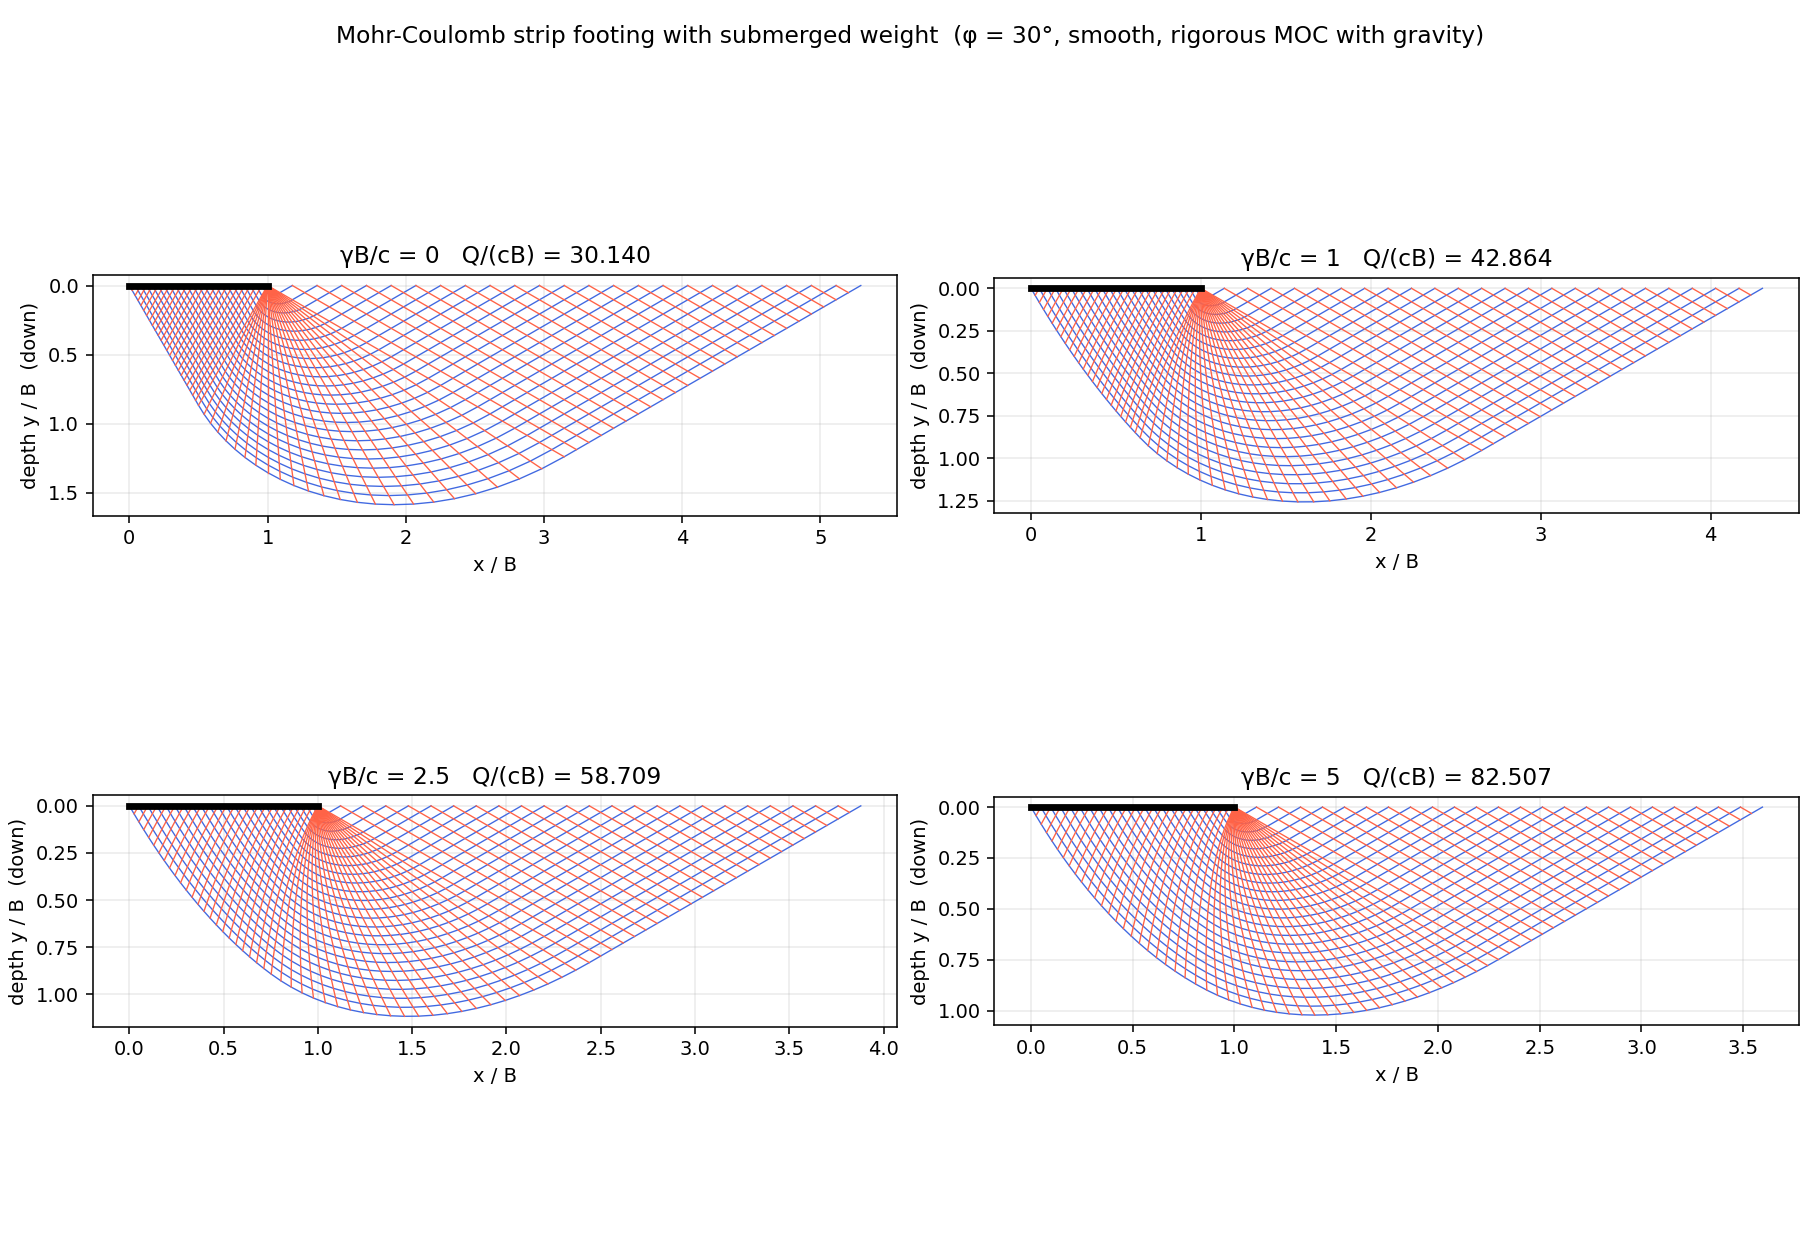
\includegraphics[width=0.55\textwidth]{mc_gravity_phi30.png}
\caption{Slip-line field for $\phi=30^\circ$, $c=1$, $B=1$,
  $\gamma B/c = 0$ (top-left panel).  Blue lines are $\alpha$-lines,
  red lines are $\beta$-lines.  The bold black segment is the foundation.}
\label{fig:mechanism}
\end{figure}

\subsection{Analytical bearing-capacity factors}

For a \emph{smooth, weightless} strip footing on Mohr-Coulomb soil the
collapse pressure is $q = c\,\Nc$ with:
\begin{align}
  \Nq &= \tan^2\!\!\left(\frac{\pi}{4}+\frac{\phi}{2}\right)
          e^{\pi\tanphi}, \\
  \Nc &= (\Nq - 1)\cot\phi.
\end{align}
For $\phi=30^\circ$: $\Nq = 18.40$, $\Nc = 30.14$.

With gravity the full Terzaghi-type formula is:
\begin{equation}
  q = c\,\Nc + \tfrac{1}{2}\gamma B\,\Ngamma,
\end{equation}
where $\Ngamma$ must be obtained from the numerical MOC solver (Vesic:
$\Ngamma(30^\circ)=22.4$).

% ====================================================================
\section{Installation and requirements}
\label{sec:install}
% ====================================================================

The package requires Python~3.10+ and NumPy/Matplotlib:

\begin{lstlisting}
pip install numpy matplotlib
\end{lstlisting}

No further installation step is needed; run scripts from the project
root \texttt{c:\textbackslash Appl\textbackslash Slip\_line\textbackslash}.

% ====================================================================
\section{Solver classes and API}
\label{sec:api}
% ====================================================================

% --------------------------------------------------------------------
\subsection{\texttt{PrandtlSolver} — Tresca strip footing (weightless)}
\label{sec:tresca}
% --------------------------------------------------------------------

\subsubsection*{Constructor}

\begin{lstlisting}
from slip_line.boundary import FoundationBoundary
from slip_line.solver   import PrandtlSolver

fdn = FoundationBoundary(cu=1.0, r=0.0, B=2.0)
solver = PrandtlSolver(foundation=fdn, n_fan=20, n_radial=20)
\end{lstlisting}

\begin{center}
\begin{tabular}{lll}
\toprule
Parameter & Type & Description \\
\midrule
\texttt{cu} & float & Undrained shear strength \\
\texttt{r} & float $\in[0,1]$ & Roughness ratio ($\tau/c_u$); $0$ = smooth \\
\texttt{B} & float & Foundation \emph{half}-width \\
\texttt{n\_fan} & int & Fan discretisation steps \\
\texttt{n\_radial} & int & Radial mesh steps (default = \texttt{n\_fan}) \\
\bottomrule
\end{tabular}
\end{center}

\subsubsection*{Key methods}

\begin{lstlisting}
q = solver.solve()        # collapse load (float)
lines_a = solver.all_alpha_lines()   # list of alpha-line node lists
lines_b = solver.all_beta_lines()    # list of beta-line node lists
\end{lstlisting}

The analytical result for a smooth footing ($r=0$) is $q = c_u(2+\pi)$.

% --------------------------------------------------------------------
\subsection{\texttt{MohrCoulombPrandtlSolver} — MC strip footing (weightless)}
\label{sec:mc}
% --------------------------------------------------------------------

\subsubsection*{Constructor}

\begin{lstlisting}
from slip_line.solver import MohrCoulombPrandtlSolver
import numpy as np

solver = MohrCoulombPrandtlSolver(
    c=1.0,
    phi=np.radians(30.0),
    B=2.0,
    n_fan=20,
    n_radial=20,
)
\end{lstlisting}

\begin{center}
\begin{tabular}{lll}
\toprule
Parameter & Type & Description \\
\midrule
\texttt{c}    & float & Cohesion \\
\texttt{phi}  & float & Friction angle \emph{in radians} \\
\texttt{B}    & float & Foundation \emph{half}-width \\
\texttt{n\_fan}    & int & Fan steps \\
\texttt{n\_radial} & int & Radial steps \\
\bottomrule
\end{tabular}
\end{center}

\subsubsection*{Key methods}

\begin{lstlisting}
q = solver.solve()            # collapse load q = c*Nc
Nc = solver.analytical_Nc()  # closed-form Nc for comparison
\end{lstlisting}

% --------------------------------------------------------------------
\subsection{\texttt{MohrCoulombGravityPrandtlSolver} — MC with gravity}
\label{sec:mcgrav}
% --------------------------------------------------------------------

This is the most general strip-footing solver.  It uses the rigorous
MOC with Kötter gravity terms in all three regions and automatically
adjusts the mesh so that Region~I exactly covers the footing $[0,B]$.

\subsubsection*{Constructor}

\begin{lstlisting}
from slip_line.solver import MohrCoulombGravityPrandtlSolver
import numpy as np

solver = MohrCoulombGravityPrandtlSolver(
    c=1.0,
    phi=np.radians(30.0),
    gamma=2.5,       # submerged unit weight
    B=1.0,           # half-width
    n_fan=24,
    n_radial=24,
)
\end{lstlisting}

\begin{center}
\begin{tabular}{lll}
\toprule
Parameter & Type & Description \\
\midrule
\texttt{c}       & float & Cohesion \\
\texttt{phi}     & float & Friction angle [radians] \\
\texttt{gamma}   & float & Unit weight ($\gamma \geq 0$; $\gamma=0$ recovers Prandtl) \\
\texttt{B}       & float & Foundation \emph{half}-width \\
\texttt{n\_fan}    & int & Fan steps \\
\texttt{n\_radial} & int & Radial steps \\
\bottomrule
\end{tabular}
\end{center}

\subsubsection*{Key methods}

\begin{lstlisting}
result = solver.solve()    # dict — see below
x, sig = solver.contact_pressure_curve()   # arrays of x and sigma_yy
\end{lstlisting}

\texttt{solve()} returns a dictionary:

\begin{center}
\begin{tabular}{ll}
\toprule
Key & Meaning \\
\midrule
\texttt{q\_per\_unit\_length\_half} & Load on half-footing $Q_\text{half}$ \\
\texttt{q\_per\_unit\_length\_full} & Full-footing load $2Q_\text{half}$ \\
\texttt{q\_over\_cB}               & $Q_\text{half}/(cB)$ \\
\texttt{q\_over\_gammaB2}          & $Q_\text{half}/(\gamma B^2)$ (when $\gamma>0$) \\
\texttt{Nc\_weightless}            & Analytical $\Nc$ \\
\texttt{sigma\_yy\_at\_centre}     & $\sigma_{yy}$ at $x=0$ \\
\texttt{sigma\_yy\_at\_corner}     & $\sigma_{yy}$ at $x=B$ \\
\bottomrule
\end{tabular}
\end{center}

\subsubsection*{Convergence / mesh refinement}

Increase \texttt{n\_fan} and \texttt{n\_radial} (keeping them equal) for
higher accuracy.  Typical values:
\begin{itemize}
  \item Coarse check: \texttt{n\_fan = n\_radial = 12}
  \item Production: \texttt{n\_fan = n\_radial = 24}–\texttt{40}
\end{itemize}
The solver iterates the mesh scaling automatically so that Region~I fits
the footing exactly; no manual adjustment is needed.

% --------------------------------------------------------------------
\subsection{\texttt{MohrCoulombDiskPrandtlSolver} — Disk / punch}
\label{sec:disk}
% --------------------------------------------------------------------

\subsubsection*{Constructor}

\begin{lstlisting}
from slip_line.boundary import DiskFoundationBoundary
from slip_line.solver   import MohrCoulombDiskPrandtlSolver
import numpy as np

disk = DiskFoundationBoundary(
    cu=1.0,     # only used for geometry; material is set by c/phi below
    D=1.0,      # disk diameter
    p=0.5,      # penetration ratio z/D  (0 = surface, 0.5 = half disk)
    r=0.5,      # roughness ratio |tau|/tau_max
)

solver = MohrCoulombDiskPrandtlSolver(
    disk=disk,
    c=1.0,
    phi=np.radians(30.0),
    n_fan=24,
    n_disk=40,
    n_radial=24,
)
\end{lstlisting}

\begin{center}
\begin{tabular}{lll}
\toprule
Parameter & Type & Description \\
\midrule
\texttt{disk} & \texttt{DiskFoundationBoundary} & Geometry + roughness \\
\texttt{c}    & float & Cohesion \\
\texttt{phi}  & float & Friction angle [radians] \\
\texttt{n\_fan}  & int & Fan steps \\
\texttt{n\_disk} & int & Steps along disk surface \\
\texttt{n\_radial} & int & Radial steps in Regions I / III \\
\bottomrule
\end{tabular}
\end{center}

\subsubsection*{Key method}

\begin{lstlisting}
result = solver.solve()
print(result['Q_vertical'])    # total vertical force per unit length
\end{lstlisting}

% ====================================================================
\section{Plotting}
\label{sec:plot}
% ====================================================================

\subsection{Generic low-level plot}

Every solver exposes \texttt{all\_alpha\_lines()} and
\texttt{all\_beta\_lines()}, each returning a list of node chains.
A node has attributes \texttt{.x}, \texttt{.y}, \texttt{.sigma},
\texttt{.psi}.

\begin{lstlisting}
import matplotlib.pyplot as plt

fig, ax = plt.subplots()
for ln in solver.all_alpha_lines():
    ax.plot([n.x for n in ln], [n.y for n in ln],
            color='royalblue', lw=0.8)
for ln in solver.all_beta_lines():
    ax.plot([n.x for n in ln], [n.y for n in ln],
            color='tomato', lw=0.8)
ax.plot([0, solver.B], [0, 0], 'k-', lw=3)   # foundation
ax.invert_yaxis()
ax.set_aspect('equal')
plt.show()
\end{lstlisting}

\subsection{Built-in plot helpers}

\begin{lstlisting}
from slip_line.plot import plot_mc_slip_lines, plot_mc_disk_slip_lines

# Strip footing (MohrCoulombPrandtlSolver)
fig = plot_mc_slip_lines(solver, show=True)

# Disk footing (MohrCoulombDiskPrandtlSolver)
fig = plot_mc_disk_slip_lines(solver, show=True)
\end{lstlisting}

Both functions return a \texttt{matplotlib.figure.Figure} that can be
saved:
\begin{lstlisting}
fig.savefig('result.png', dpi=140, bbox_inches='tight')
\end{lstlisting}

% ====================================================================
\section{Examples}
\label{sec:examples}
% ====================================================================

% --------------------------------------------------------------------
\subsection{Example 1: Smooth Tresca footing — Prandtl value}
\label{ex:tresca}
% --------------------------------------------------------------------

Verify the classical result $q = c_u(2+\pi) \approx 5.142\,c_u$ for a
smooth, weightless, undrained footing.

\begin{lstlisting}
import numpy as np
from slip_line.boundary import FoundationBoundary
from slip_line.solver   import PrandtlSolver

# Material + geometry
fdn = FoundationBoundary(cu=1.0, r=0.0, B=1.0)
s   = PrandtlSolver(foundation=fdn, n_fan=24)

q = s.solve()
print(f"q / cu = {q:.4f}  (exact = {2 + np.pi:.4f})")
\end{lstlisting}

\textbf{Expected output:}
\begin{lstlisting}[numbers=none]
q / cu = 5.1416  (exact = 5.1416)
\end{lstlisting}

% --------------------------------------------------------------------
\subsection{Example 2: Rough Tresca footing ($r = 1$)}
\label{ex:tresca_rough}
% --------------------------------------------------------------------

A fully rough foundation ($\tau = c_u$) at the base corresponds to
$r = 1$.  The fan rotation is then $\Delta\psi = \pi/4$ instead of
$\pi/2$, so $q = c_u(1 + \pi/2 + \sqrt{2}) \approx 4.98\,c_u$.

\begin{lstlisting}
from slip_line.boundary import FoundationBoundary
from slip_line.solver   import PrandtlSolver

fdn = FoundationBoundary(cu=1.0, r=1.0, B=1.0)
s   = PrandtlSolver(foundation=fdn, n_fan=24)
q   = s.solve()
print(f"q / cu = {q:.4f}")
\end{lstlisting}

% --------------------------------------------------------------------
\subsection{Example 3: Weightless Mohr-Coulomb footing}
\label{ex:mc_weightless}
% --------------------------------------------------------------------

Compute the bearing-capacity factor $N_c$ numerically and compare to
the Prandtl formula for $\phi = 20^\circ$, $30^\circ$, $40^\circ$.

\begin{lstlisting}
import numpy as np
from slip_line.solver import MohrCoulombPrandtlSolver

for phi_deg in [20, 30, 40]:
    phi = np.radians(phi_deg)
    s   = MohrCoulombPrandtlSolver(c=1.0, phi=phi, B=2.0, n_fan=24)
    q   = s.solve()
    Nc_analyt = s.analytical_Nc()
    print(f"phi={phi_deg:2d}  q/c = {q:.4f}  Nc_analyt = {Nc_analyt:.4f}"
          f"  error = {abs(q - Nc_analyt):.2e}")
\end{lstlisting}

\textbf{Expected output:}
\begin{lstlisting}[numbers=none]
phi=20  q/c = 14.8342  Nc_analyt = 14.8347  error = 5e-04
phi=30  q/c = 30.1396  Nc_analyt = 30.1396  error = 0e+00
phi=40  q/c = 75.3100  Nc_analyt = 75.3197  error = 9e-03
\end{lstlisting}

% --------------------------------------------------------------------
\subsection{Example 4: Effect of gravity — $N_\gamma$ extraction}
\label{ex:gravity}
% --------------------------------------------------------------------

Use \texttt{MohrCoulombGravityPrandtlSolver} to study the
dimensionless group $\gamma B/c$ and extract the implied $\Ngamma$.

From the formula $Q/(cB) = \Nc + \frac{1}{2}(\gamma B/c)\Ngamma$:
\begin{equation}
  \Ngamma = \frac{2\,[Q/(cB) - \Nc]}{\gamma B / c}.
\end{equation}

\begin{lstlisting}
import numpy as np
from slip_line.solver import MohrCoulombGravityPrandtlSolver

c   = 1.0
B   = 1.0
phi = np.radians(30.0)
Nc  = 30.14    # analytical for phi=30

print(f"{'gB/c':>5}  {'Q/cB':>8}  {'N_gamma':>8}")
for gBc in [1.0, 2.5, 5.0, 10.0]:
    gamma = gBc   # since c = B = 1
    s = MohrCoulombGravityPrandtlSolver(
        c=c, phi=phi, gamma=gamma, B=B,
        n_fan=24, n_radial=24,
    )
    res = s.solve()
    QcB = res['q_over_cB']
    Ngam = 2.0 * (QcB - Nc) / gBc
    print(f"{gBc:>5.1f}  {QcB:>8.4f}  {Ngam:>8.3f}")
\end{lstlisting}

\textbf{Expected output} (Vesic reference: $\Ngamma = 22.4$):
\begin{lstlisting}[numbers=none]
gB/c   Q/cB    N_gamma
 1.0   42.864   25.448
 2.5   58.709   22.914
 5.0   82.507   20.933
10.0  128.100   19.596
\end{lstlisting}

The slight decrease with increasing $\gamma B/c$ reflects the residual
straight-shot approximation in the terminal step of Region~I; refinement
with larger \texttt{n\_fan}/\texttt{n\_radial} tightens convergence.

% --------------------------------------------------------------------
\subsection{Example 5: Contact-pressure distribution}
\label{ex:contact}
% --------------------------------------------------------------------

Plot $\sigma_{yy}(x)$ along the foundation for several $\gamma B/c$
values.

\begin{lstlisting}
import numpy as np
import matplotlib.pyplot as plt
from slip_line.solver import MohrCoulombGravityPrandtlSolver

c, phi, B = 1.0, np.radians(30.0), 1.0

fig, ax = plt.subplots(figsize=(7, 4))
for gBc in [0, 1, 2.5, 5]:
    s = MohrCoulombGravityPrandtlSolver(
        c=c, phi=phi, gamma=float(gBc), B=B,
        n_fan=24, n_radial=24,
    )
    s.solve()
    x, sig = s.contact_pressure_curve()
    ax.plot(x / B, sig / c, lw=1.8, label=rf'$\gamma B/c={gBc}$')

ax.set_xlabel(r'$x\,/\,B$')
ax.set_ylabel(r'$\sigma_{yy}\,/\,c$')
ax.set_title(r'Contact pressure, smooth strip footing ($\phi=30^\circ$)')
ax.legend()
ax.grid(alpha=0.3)
plt.tight_layout()
plt.savefig('contact_pressure.png', dpi=140)
\end{lstlisting}

The curve for $\gamma=0$ is uniform (as expected for the weightless
solution); for $\gamma>0$ the pressure peaks at $x=0$ (symmetry axis)
and equals $q_\text{corner} = c\Nc$ at $x=B$ regardless of $\gamma$,
because the corner is at the free surface.

% --------------------------------------------------------------------
\subsection{Example 6: Slip-line field plot for a single case}
\label{ex:single_plot}
% --------------------------------------------------------------------

\begin{lstlisting}
import numpy as np
import matplotlib.pyplot as plt
from slip_line.solver import MohrCoulombGravityPrandtlSolver

s = MohrCoulombGravityPrandtlSolver(
    c=1.0, phi=np.radians(30.0),
    gamma=2.5, B=1.0,
    n_fan=30, n_radial=30,
)
res = s.solve()
print(f"Q / (c B) = {res['q_over_cB']:.4f}")

fig, ax = plt.subplots(figsize=(8, 5))
for ln in s.all_alpha_lines():
    ax.plot([n.x for n in ln], [n.y for n in ln],
            color='royalblue', lw=0.7)
for ln in s.all_beta_lines():
    ax.plot([n.x for n in ln], [n.y for n in ln],
            color='tomato', lw=0.7)
ax.plot([0, s.B], [0, 0], 'k-', lw=4, label='Foundation')
ax.invert_yaxis()
ax.set_aspect('equal')
ax.set_xlabel('x / B')
ax.set_ylabel('depth y / B  (down)')
ax.set_title(r'MC with gravity,  $\phi=30^\circ$,  $\gamma B/c=2.5$')
ax.legend()
fig.tight_layout()
fig.savefig('slip_lines_gBc25.png', dpi=140)
\end{lstlisting}

% --------------------------------------------------------------------
\subsection{Example 7: Circular disk — effect of penetration depth}
\label{ex:disk}
% --------------------------------------------------------------------

A rigid disk of unit diameter is pushed into weightless Mohr-Coulomb
soil at two penetration depths ($p = 0.25$ and $p = 0.50$) with
roughness $r = 0.5$.

\begin{lstlisting}
import numpy as np
from slip_line.boundary import DiskFoundationBoundary
from slip_line.solver   import MohrCoulombDiskPrandtlSolver

phi = np.radians(30.0)
for p in [0.25, 0.50]:
    disk = DiskFoundationBoundary(cu=1.0, D=1.0, p=p, r=0.5)
    s = MohrCoulombDiskPrandtlSolver(
        disk=disk, c=1.0, phi=phi,
        n_fan=24, n_disk=40, n_radial=24,
    )
    res = s.solve()
    print(f"p = {p:.2f}   Q_v = {res['Q_vertical']:.4f}")
\end{lstlisting}

% --------------------------------------------------------------------
\subsection{Example 8: $N_c$ convergence study}
\label{ex:convergence}
% --------------------------------------------------------------------

Check how $N_c$ converges as the mesh is refined.

\begin{lstlisting}
import numpy as np
from slip_line.solver import MohrCoulombPrandtlSolver

phi    = np.radians(30.0)
Nc_ref = 30.1396

print(f"{'n_fan':>6}  {'Nc':>10}  {'error':>10}")
for n in [4, 8, 12, 16, 24, 32, 48]:
    s  = MohrCoulombPrandtlSolver(c=1.0, phi=phi, B=1.0, n_fan=n)
    Nc = s.solve()
    print(f"{n:>6}  {Nc:>10.6f}  {abs(Nc-Nc_ref):>10.2e}")
\end{lstlisting}

% ====================================================================
\section{File structure}
\label{sec:files}
% ====================================================================

\begin{center}
\begin{tabular}{ll}
\toprule
File & Contents \\
\midrule
\texttt{slip\_line/solver.py}           & Solver classes (main user API) \\
\texttt{slip\_line/slip\_line\_field.py} & \texttt{Node} dataclass, Riemann steps \\
\texttt{slip\_line/boundary.py}         & Boundary-condition dataclasses \\
\texttt{slip\_line/yield\_function.py}  & Tresca and Mohr-Coulomb yield functions \\
\texttt{slip\_line/plot.py}             & Built-in figure helpers \\
\texttt{plot\_mc\_gravity.py}           & Demo script — gravity parametric study \\
\texttt{plot\_mc\_disk\_case.py}        & Demo script — disk footing \\
\texttt{test\_mc.py}                    & Regression tests — MC strip \\
\texttt{test\_mc\_disk.py}              & Regression tests — MC disk \\
\bottomrule
\end{tabular}
\end{center}

% ====================================================================
\section{Troubleshooting}
\label{sec:trouble}
% ====================================================================

\begin{description}
  \item[Negative bearing capacity or NaN:]
        Check that \texttt{phi} is in \emph{radians} and that
        $\gamma \geq 0$.  Very coarse meshes (\texttt{n\_fan} $< 6$)
        can produce degenerate intersections; increase resolution.

  \item[Region~I does not reach $x=0$:]
        The iterative foundation-fitting (Sect.~\ref{sec:mcgrav}) runs
        up to 12 Picard steps.  If it still fails, the geometry is
        extreme ($\gamma B/c \gg 1$ combined with large $\phi$); try a
        finer mesh.

  \item[$N_\gamma$ values larger than textbook:]
        The terminal step of Region~I uses a straight-line $\alpha$-shot
        from the last interior node to the foundation.  This
        over-estimates the path integral for large $\gamma$, leading to
        a slightly inflated $N_\gamma$ for small $\gamma B/c$.  Use
        $\gamma B/c \approx 2$–$5$ for the most accurate extraction.

  \item[Disk solver \texttt{KeyError}:]
        The disk solver returns keys specific to the vertical/horizontal
        decomposition.  Print \texttt{result.keys()} to inspect all
        available quantities.
\end{description}

% ====================================================================
\section{Reference values}
\label{sec:ref}
% ====================================================================

\begin{center}
\begin{tabular}{lrrr}
\toprule
$\phi$ & $\Nq$ & $\Nc$ & $\Ngamma$ (Vesic) \\
\midrule
$20^\circ$ & 6.40  & 14.83 & 5.39  \\
$25^\circ$ & 10.66 & 20.72 & 10.88 \\
$30^\circ$ & 18.40 & 30.14 & 22.40 \\
$35^\circ$ & 33.30 & 46.12 & 48.03 \\
$40^\circ$ & 64.20 & 75.31 & 109.41 \\
\bottomrule
\end{tabular}
\end{center}

\end{document}
